% ============================
% DOCUMENT SETUP
% ============================
\documentclass[12pt]{article}

% ============================
% PACKAGES
% ============================

% --- Matemáticas ---
\usepackage{amsmath, amsthm, amssymb, amsfonts, amsbsy, amscd}

% --- Tablas y Figuras ---
\usepackage{graphicx} % Para incluir imágenes
\usepackage{tabularx} % Tablas de ancho automático
\usepackage{float}    % Mejor control de ubicación de figuras/tablas
\usepackage{booktabs} % Mejor estilo para tablas
\usepackage{multirow} % Combinar filas en tablas
\usepackage{diagbox}  % Crear diagonales en tablas
\usepackage{subfig}   % Subfiguras
\usepackage{caption}  % Personalizar leyendas

% --- Tipografía y Formato ---
\usepackage{times}       % Fuente Times New Roman
\usepackage{setspace}    % Espaciado
\usepackage{microtype}   % Mejoras tipográficas
\usepackage[none]{hyphenat} % Evitar partición de palabras

% --- Geometría ---
\usepackage[letterpaper, bottom=2.5cm, top=2.5cm, right=2.5cm, left=3cm, headsep=1.5cm]{geometry}

% --- Encabezados y Pies de Página ---
\usepackage{fancyhdr}
\usepackage{lastpage}

% --- Enumeraciones ---
\usepackage{enumitem} % Mejor control sobre listas

% --- Otros ---
\usepackage{tikz}     % Para gráficos vectoriales
\usepackage{cancel}   % Para tachar en fórmulas
\usepackage{cite}     % Para manejo de citas
\usepackage{chicago}  % Estilo de bibliografía Chicago

% --- Enlaces e Hipervínculos ---
\usepackage{hyperref}
\hypersetup{
    colorlinks=true,
    breaklinks=true,
    linkcolor=black,
    citecolor=blue,
    filecolor=magenta,
    urlcolor=blue
}

\usepackage{pgfplots}
\pgfplotsset{compat=1.18} % Asegúrate de tener una versión compatible
\usepackage{pgfplotstable}

% ============================
% DEFINICIONES
% ============================

\providecommand{\abs}[1]{\lvert#1\rvert}

\DeclareMathOperator*{\argmin}{arg\,min} % Operador argmin
\DeclareMathOperator*{\argmax}{arg\,max} % Operador argmax

\renewcommand*\contentsname{Index} % Cambiar nombre de tabla de contenidos
\setlength{\footskip}{45pt} % Distancia pie de página
\setlength{\parindent}{0pt} % Sin sangría en párrafos

% ============================
% DOCUMENTO
% ============================

\title{\textbf{Homework 3, Final Report\\ \vspace{0.5cm} \\ Finite Elements}}
\def\footerlogo{LOGO_UNIVERSIDAD.jpg} % Logo para el pie de página
\date{\textbf{May 26, 2025}}

\begin{document}
\makeatletter
\begin{titlepage}
    \begin{center}
        \vspace{2cm}
        \includegraphics[width=0.8\linewidth]{LOGO_UNIVERSIDAD.jpg}\\[10ex]
        
        \rule{\textwidth}{1pt} \\[2ex]
        {\LARGE \textbf{Homework 3, Final Report\\ \vspace{0.5cm} Finite Elements}}\\[2ex]
        \rule{\textwidth}{1pt} \\[10ex]

        \vfill

        \begin{flushright}
            \textbf{Professor:\\
             Jose A. Abell} \\[0.3cm]
            \textbf{Students: \\
            Bernardo Caprile\\
            Pedro Valenzuela} \\[0.3cm]
        \end{flushright}
        
        \vspace*{1cm}
        {\normalsize \@date}
    \end{center}
\end{titlepage}
\makeatother


\pagestyle{fancy}
\fancyhf{}
\rhead{\shorttitle}


%\lhead{Guides and tutorials}
\rfoot{\thepage}
\lhead{Finite Elements} 
\rhead{\includegraphics[width=0.25\linewidth]{LOGO_UNIVERSIDAD.jpg}} % For header of the document
\renewcommand{\footrulewidth}{0.5pt}

\tableofcontents

%% If you write a long report, add list of figures and tables and start reporting on new page
%\listoffigures
%\listoftables
%\newpage
\thispagestyle{empty}
\newpage
\spacing{1.15}
\setcounter{page}{1}

\newpage
\section*{GitHub Repository}

The code and data for this project are available on GitHub at the following link:
\begin{center}
    \url{https://github.com/berckanala/01-Finite-Element}
\end{center}


\newpage
\section{Stress Analysis (Part B)}

\subsection{Introduction}
This study uses the finite element method to analyze maximum principal stresses in a part with a stress concentration. Four mesh sizes, two refinement strategies (global and local), and two element types (Quad4 and Quad9) are compared, resulting in 16 simulations. The goal is to evaluate how these factors affect stress distribution, particularly near the critical region, and to observe convergence with mesh refinement.
\\
\\
\newpage
\subsection{Results}

\subsubsection{Quad4 global refinement elements}

\begin{figure}[H]
    \centering
    \begin{minipage}{0.48\textwidth}
        \centering
        \includegraphics[width=\textwidth]{../resultados/Quad_4_Global_refinement_case_1_-_Maximum_Principal_Stress_σ1.png}
        \caption{Quad4 Case 1 – Global Refinement}
        \label{fig:quad4_results_global1}
    \end{minipage}
    \hfill
    \begin{minipage}{0.48\textwidth}
        \centering
        \includegraphics[width=\textwidth]{../resultados/Quad_4_Global_refinement_case_2_-_Maximum_Principal_Stress_σ1.png}
        \caption{Quad4 Case 2 – Global Refinement}
        \label{fig:quad4_results_global2}
    \end{minipage}
\end{figure}

\begin{figure}[H]
    \centering
    \begin{minipage}{0.48\textwidth}
        \centering
        \includegraphics[width=\textwidth]{../resultados/Quad_4_Global_refinement_case_3_-_Maximum_Principal_Stress_σ1.png}
        \caption{Quad4 Case 3 – Global Refinement}
        \label{fig:quad4_results_global3}
    \end{minipage}
    \hfill
    \begin{minipage}{0.48\textwidth}
        \centering
        \includegraphics[width=\textwidth]{../resultados/Quad_4_Global_refinement_case_4_-_Maximum_Principal_Stress_σ1.png}
        \caption{Quad4 Case 4 – Global Refinement}
        \label{fig:quad4_results_global4}
    \end{minipage}
\end{figure}

\newpage
\subsubsection{Quad4 local refinement elements}
\begin{figure}[H]
    \centering
    \begin{minipage}{0.48\textwidth}
        \centering
        \includegraphics[width=\textwidth]{../resultados/Quad_4_Local_refinement_case_1_-_Maximum_Principal_Stress_σ1.png}
        \caption{Quad4 Case 1 – Local Refinement}
        \label{fig:quad4_results_local1}
    \end{minipage}
    \hfill
    \begin{minipage}{0.48\textwidth}
        \centering
        \includegraphics[width=\textwidth]{../resultados/Quad_4_Local_refinement_case_2_-_Maximum_Principal_Stress_σ1.png}
        \caption{Quad4 Case 2 – Local Refinement}
        \label{fig:quad4_results_local2}
    \end{minipage}
\end{figure}

\begin{figure}[H]
    \centering
    \begin{minipage}{0.48\textwidth}
        \centering
        \includegraphics[width=\textwidth]{../resultados/Quad_4_Local_refinement_case_3_-_Maximum_Principal_Stress_σ1.png}
        \caption{Quad4 Case 3 – Local Refinement}
        \label{fig:quad4_results_local3}
    \end{minipage}
    \hfill
    \begin{minipage}{0.48\textwidth}
        \centering
        \includegraphics[width=\textwidth]{../resultados/Quad_4_Local_refinement_case_4_-_Maximum_Principal_Stress_σ1.png}
        \caption{Quad4 Case 4 – Local Refinement}
        \label{fig:quad4_results_local4}
    \end{minipage}
\end{figure}

\newpage
\subsubsection{Quad9 global refinement elements}

\begin{figure}[H]
    \centering
    \begin{minipage}{0.48\textwidth}
        \centering
        \includegraphics[width=\textwidth]{../resultados/Quad_9_Global_refinement_case_1_-_Maximum_Principal_Stress_σ1.png}
        \caption{Quad9 Case 1 – Global Refinement}
        \label{fig:quad9_results_global1}
    \end{minipage}
    \hfill
    \begin{minipage}{0.48\textwidth}
        \centering
        \includegraphics[width=\textwidth]{../resultados/Quad_9_Global_refinement_case_2_-_Maximum_Principal_Stress_σ1.png}
        \caption{Quad9 Case 2 – Global Refinement}
        \label{fig:quad9_results_global2}
    \end{minipage}
\end{figure}

\begin{figure}[H]
    \centering
    \begin{minipage}{0.48\textwidth}
        \centering
        \includegraphics[width=\textwidth]{../resultados/Quad_9_Global_refinement_case_3_-_Maximum_Principal_Stress_σ1.png}
        \caption{Quad9 Case 3 – Global Refinement}
        \label{fig:quad9_results_global3}
    \end{minipage}
    \hfill
    \begin{minipage}{0.48\textwidth}
        \centering
        \includegraphics[width=\textwidth]{../resultados/Quad_9_Global_refinement_case_4_-_Maximum_Principal_Stress_σ1.png}
        \caption{Quad9 Case 4 – Global Refinement}
        \label{fig:quad9_results_global4}
    \end{minipage}
\end{figure}

\newpage
\subsubsection{Quad9 local refinement elements}

\begin{figure}[H]
    \centering
    \begin{minipage}{0.48\textwidth}
        \centering
        \includegraphics[width=\textwidth]{../resultados/Quad_9_Local_refinement_case_1_-_Maximum_Principal_Stress_σ1.png}
        \caption{Quad9 Case 1 – Local Refinement}
        \label{fig:quad9_results_local1}
    \end{minipage}
    \hfill
    \begin{minipage}{0.48\textwidth}
        \centering
        \includegraphics[width=\textwidth]{../resultados/Quad_9_Local_refinement_case_2_-_Maximum_Principal_Stress_σ1.png}
        \caption{Quad9 Case 2 – Local Refinement}
        \label{fig:quad9_results_local2}
    \end{minipage}
\end{figure}

\begin{figure}[H]
    \centering
    \begin{minipage}{0.48\textwidth}
        \centering
        \includegraphics[width=\textwidth]{../resultados/Quad_9_Local_refinement_case_3_-_Maximum_Principal_Stress_σ1.png}
        \caption{Quad9 Case 3 – Local Refinement}
        \label{fig:quad9_results_local3}
    \end{minipage}
    \hfill
    \begin{minipage}{0.48\textwidth}
        \centering
        \includegraphics[width=\textwidth]{../resultados/Quad_9_Local_refinement_case_4_-_Maximum_Principal_Stress_σ1.png}
        \caption{Quad9 Case 4 – Local Refinement}
        \label{fig:quad9_results_local4}
    \end{minipage}
\end{figure}

\newpage
\subsection{Results Summary and Discussion }

The following tables summarize the maximum principal stress values obtained from the finite element simulations using Quad4 and Quad9 elements. For each element type, results are presented under two mesh refinement strategies (global and local) and across four mesh sizes. These values help evaluate the convergence behavior and the influence of element type and mesh refinement on the accuracy of stress predictions, particularly near regions of stress concentration.

\begin{table}[H]
\centering
\begin{minipage}{0.48\textwidth}
\centering
\begin{tabular}{|c|c|c|}
\hline
\textbf{Element Type} & \textbf{Case} & \textbf{Max $\sigma_1$ [MPa]} \\
\hline
Quad4 & 1 & 353.84 \\
Quad4 & 2 & 359.28 \\
Quad4 & 3 & 375.95 \\
Quad4 & 4 & 375.71 \\
\hline
\end{tabular}
\caption{Quad4 Elements – Global Refinement}
\label{tab:quad4_global}
\end{minipage}
\hfill
\begin{minipage}{0.48\textwidth}
\centering
\begin{tabular}{|c|c|c|}
\hline
\textbf{Element Type} & \textbf{Case} & \textbf{Max $\sigma_1$ [MPa]} \\
\hline
Quad4 & 1 & 330.87 \\
Quad4 & 2 & 338.38 \\
Quad4 & 3 & 355.20 \\
Quad4 & 4 & 358.17 \\
\hline
\end{tabular}
\caption{Quad4 Elements – Local Refinement}
\label{tab:quad4_local}
\end{minipage}
\end{table}

In the case of Quad4 elements, the maximum principal stress values exhibit a clear convergence trend as the mesh is refined. The use of local refinement leads to slightly lower and more stable stress values compared to global refinement, especially in finer meshes. This suggests that concentrating mesh density in regions of high stress is more effective than refining the entire domain uniformly.

\begin{table}[H]
\centering
\begin{minipage}{0.48\textwidth}
\centering
\begin{tabular}{|c|c|c|}
\hline
\textbf{Element Type} & \textbf{Case} & \textbf{Max $\sigma_1$ [MPa]} \\
\hline
Quad9 & 1 & 353.83 \\
Quad9 & 2 & 359.28 \\
Quad9 & 3 & 375.94 \\
Quad9 & 4 & 375.71 \\
\hline
\end{tabular}
\caption{Quad9 Elements – Global Refinement}
\label{tab:quad9_global}
\end{minipage}
\hfill
\begin{minipage}{0.48\textwidth}
\centering
\begin{tabular}{|c|c|c|}
\hline
\textbf{Element Type} & \textbf{Case} & \textbf{Max $\sigma_1$ [MPa]} \\
\hline
Quad9 & 1 & 330.86 \\
Quad9 & 2 & 338.38 \\
Quad9 & 3 & 355.20 \\
Quad9 & 4 & 358.17 \\
\hline
\end{tabular}
\caption{Quad9 Elements – Local Refinement}
\label{tab:quad9_local}
\end{minipage}
\end{table}

In the case of Quad9 elements, the maximum principal stress values demonstrate consistent convergence trend as the mesh is refined. Local refinement leads to slightly lower stress values than global refinement, particularly in the finer mesh cases, indicating improved accuracy around stress concentration zones.

\begin{figure}[H]
    \centering
    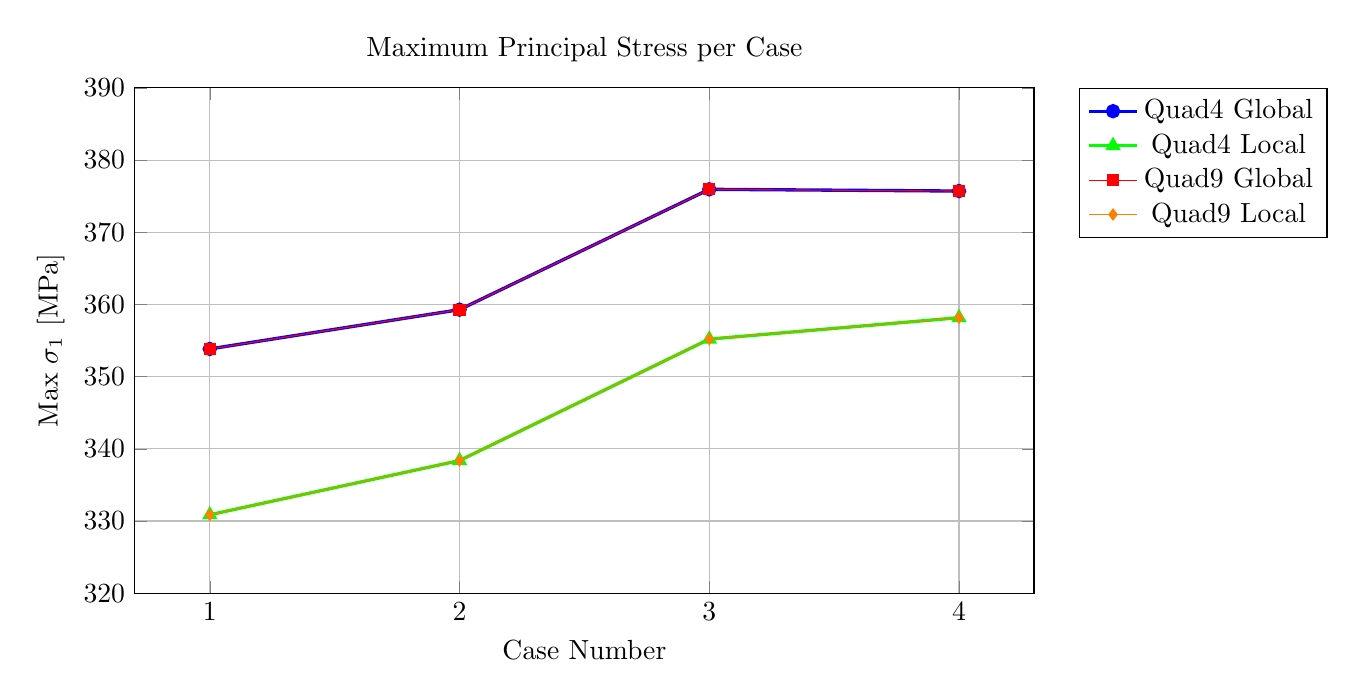
\begin{tikzpicture}
    \begin{axis}[
        width=13cm,
        height=8cm,
        xlabel={Case Number},
        ylabel={Max $\sigma_1$ [MPa]},
        title={Maximum Principal Stress per Case},
        legend style={at={(1.05,1)}, anchor=north west},
        xtick={1,2,3,4},
        grid=both,
        ymin=320, ymax=390
    ]

    % Quad4 Global
    \addplot[line width=1.2pt, color=blue, mark=*] coordinates {
        (1, 353.84)
        (2, 359.28)
        (3, 375.95)
        (4, 375.71)
    };
    \addlegendentry{Quad4 Global}

    % Quad4 Local
    \addplot[line width=1.2pt, color=green, mark=triangle*] coordinates {
        (1, 330.87)
        (2, 338.38)
        (3, 355.20)
        (4, 358.17)
    };
    \addlegendentry{Quad4 Local}

    % Quad9 Global
    \addplot[color=red, mark=square*] coordinates {
        (1, 353.83)
        (2, 359.28)
        (3, 375.94)
        (4, 375.71)
    };
    \addlegendentry{Quad9 Global}

    % Quad9 Local
    \addplot[color=orange, mark=diamond*] coordinates {
        (1, 330.86)
        (2, 338.38)
        (3, 355.20)
        (4, 358.17)
    };
    \addlegendentry{Quad9 Local}

    \end{axis}
    \end{tikzpicture}
    \caption{Maximum principal stress for each refinement case and element type}
    \label{fig:max_stress_comparison}
\end{figure}

When comparing the results from Quad4 and Quad9 elements, it is evident that both types are capable of capturing the overall behavior of the principal stress distribution. However, Quad9 elements, being higher-order, exhibit smoother and more accurate convergence, especially in regions of stress concentration. They can deliver more precise results with fewer elements, making them computationally efficient when combined with properly applied local mesh refinement.

On the other hand, Quad4 elements are simpler and require less computational effort per element, making them suitable for preliminary analyses or when resources are limited. However, their accuracy relies more heavily on mesh density, and they benefit significantly from local refinement near critical areas.

\newpage
\section{Design Modification and Stress Redistribution (Part C)}

For us to optimize the stresses of the profile, first we divided the section in two parts, Steel 1 and Steel 2. Steel 1 is the part closer to the supports (left side of the figure), while Steel 2 is the part farther away from them (right side of the figure). The sections can be seen i the following figure:

\begin{figure}[H]
    \centering
    \includegraphics[width=0.8\textwidth]{image.png}
    \caption{Gmsh of the profile}
    \label{fig:modified_profile_stress}
\end{figure}

To improve its performance, we modified the cross section by reducing 5\% of the material from the region Steel 1 and redistributing it to Steel 2. Although this approach may initially seem counterintuitive, it increases the mass of the outer region, generating a greater moment due to the self-weight, which pushes the profile downward.

Since the applied force tends to lift the profile upward, this redistribution acts as a counterbalance, reducing the upward deflection and stabilizing the system. As a result, the internal stresses are reduced. This modification was analyzed using the 9L4 model to ensure accurate results.

\newpage

The following figures shows the stresses obtained from the 9L4 model (Quad9, local refinement, case 4), which was used for the profile modification. This includes both the original and the modified cases.

\begin{figure}[H]
    \centering
    \begin{minipage}{0.48\textwidth}
        \centering
        \includegraphics[width=\textwidth]{../resultados/Quad_9_Local_refinement_case_4_-_Maximum_Principal_Stress_σ1.png}
        \caption{Original case – Quad9 Local Case 4}
        \label{fig:quad9_local4_original}
    \end{minipage}
    \hfill
    \begin{minipage}{0.48\textwidth}
        \centering
        \includegraphics[width=\textwidth]{../resultados/Perfil_optimizado_-_Maximum_Principal_Stress_σ1.png}
        \caption{Modified case – Quad9 Local Case 4}
        \label{fig:quad9_local4_modified}
    \end{minipage}
\end{figure}

In this case, the maximum principal stress in the original configuration is 358.17 MPa, while in the modified configuration it is 355.41 MPa, showing a reduction of approximately 3 MPa.



\newpage
\section{Summary Essay (Part D)}

This assignment provided insights into how mesh refinement and local geometry modifications influence the accuracy and interpretation of stress analysis using the finite element method (FEM). One of the most important lessons was understanding the trade-off between mesh density and computational efficiency. As the mesh becomes finer, especially in critical regions where stress concentrations occur, the predicted stress values become more accurate and reliable. Local mesh refinement proved particularly effective, offering improved resolution where needed without excessively increasing the global element count.

Through comparative simulations using both Quad4 and Quad9 elements under global and local refinement strategies, we observed that higher-order elements such as Quad9 deliver smoother and more precise results with fewer elements, especially when combined with local refinement. This underscored the importance of selecting appropriate element types and refinement techniques based on the goals of the analysis and available computational resources.

A key part of the assignment involved applying a local geometric modification: redistributing material from the region directly over the supports to the area farther away. Although initially counterintuitive, this modification effectively reduced the maximum principal stress. By increasing the moment generated by self-weight, the profile counteracted the upward bending caused by external loads. This highlighted how even small geometric changes can significantly influence stress distribution and structural behavior.

Finally, the process emphasized the iterative nature of FEM modeling. From mesh generation and boundary condition definition to result interpretation, careful attention to detail is essential. Errors in geometry, meshing, or assumptions can lead to misleading conclusions. Overall, this assignment deepened my understanding of how thoughtful modeling strategies and refinement choices directly impact the fidelity and usefulness of FEM analyses in structural engineering contexts.

\end{document}

